% Introdução: cenario, motivacao, problema, solucoes atuais, escopo do trabalho, lista de contribuicoes, organizacao do resto do artigo. 
% Chapter Structure
% 	Motivation
% 	Problems Statement
%	Contributions
% 	Dissertation Organization
\chapter{Introduction}
\label{ch:introduction}

\begin{quotation}[]{Chico Xavier}
Though nobody can go back and make a new beginning, anyone can start over and make a new ending.
\end{quotation}


\section{Motivation}
\label{sc:motivation}

Traditionally, cyber defense methods can be effective against ordinary and conventional types of attacks, yet may fail against innovative malicious techniques \cite{lakhina2005mining}. In order to be able to detect and avoid novel attacks and their variations, it is necessary to develop or improve techniques to achieve efficiency on resource consumption, processing capacity and response time. Moreover, it is crucial to obtain high detection accuracy and capacity to detect variations of malicious patterns. Recently, signal processing schemes have being applied to the detection of malicious traffic in computer networks \cite{Lu2009,Huang2009,Zonglin2009,david2011blind,da2012improved,tenorio2013greatest}, showing advances in network traffic analysis.

Information security may consist of both technical and procedural aspects. The former includes equipment and security systems, while the latter corresponds to security rules and recommendations. Intrusion detection and intrusion prevention systems are security systems used, respectively, to detect (passively) and prevent (proactively) threats to computer systems and computer networks. Such systems can work in the following fashions: signature-based, anomaly-based or hybrid \cite{Huang2009,mudzingwa2012study}. Additionally, anomaly detection techniques can be categorized in classification, statistical, information theory and clustering based, according to \cite{bhuyan2014network,ahmed2016survey,osanaiye2016distributed}.

Cloud computing is a new rapidly evolving paradigm in the world of distributed networking and computation. The basic features of the cloud environment is providing the elastic, on-demand and secure services for the end-users. While the first two requirements are rather well conceptualized and supported by the majority of the cloud platforms in use, security is a serious concern of the cloud providers and governmental organizations as well as academia and research community \cite{csa2016,higashi2015,gartner2015}. Although for the small and medium-sized enterprises (SME) the cloud environment is often the most cost-effective and easily scalable solution, the security and privacy of the sensitive data in cloud platforms are also not fully conceptualized leading to obscure and incomplete security paradigms and solutions.

Additional security issues and requirements have to be considered when mobile clients are actively used in corporate cloud environment \cite{yovel2014}. Today more and more organizations and enterprises are functioning in the Bring-Your-Own-Device (BYOD) paradigm. The uncontrolled usage of the mobile devices represents a serious risk to the development of secure SME cloud platforms being the bottleneck of the corporate information security system (ISS). While the enterprise cloud infrastructure based on the web interface can be protected by powerful third-party services, the corporate mobile client is usually light-weighted and generally less protected. 

The protection scheme used on a mobile device should be both computationally secure as well as resource-constrained due to battery power limitations \cite{khan2015cloud}. Therefore, encrypting files and generating keys on a mobile device is not considered a good solution. On the other hand, the protection schemes with good computational qualities lack the security analysis in many cases \cite{khan2014bss}. The common practice is the shadow user activities monitoring \cite{yovel2014}. However, the mobile device usage stays unprotected in all the proposed scenarios while in offline mode. When the mobile client goes offline with the sensitive corporate data on board all powerful cloud-based tools cannot help and the mobile client has to secure itself with its own limited resources. Moreover, due to the resources constraint, there is a crucial difference in strategy of online and offline mode protection. For example, offline mode does not allow performing the extensive computation and encryption on the mobile device.

The field of Mobile Money Transfer (MMT) is a growing market segment and has been motivating investiments into security defense and fraud detection. Obtaining access to data sets of mobile transactions for research is a very hard task due to the intrinsic private nature of such transactions. Scientists and researchers must today spend time and effort in obtaining permits and access to relevant data sets before they can research on such data set. However, PaySim is a financial simulator that simulates mobile money transactions based on an original dataset and provides a synthetic dataset as an approach to such a problem.\footnote{https://www.kaggle.com/ntnu-testimon/paysim1}

Despite the actual high availability of information, the relevant information of some observations is generally of under much reduced dimensionality compared to available data sets. The extraction of relevant information by identifying the generating causes within classes of signals is useful for classification problems and for security analysis. Big data analytics require techniques to deal with multidimensional data, making sense of strucutre and relationship of many dimensions. Dictionary learning is a signal processing technique based on the principle that some observations can be described by a sparse subset of atoms taken from a redundant dictionary, which represents the causes of some observations of the world. Dictionary Learning is a signal processing technique for sparse representation of signals as basis vectors, learning the representations from training data, as dictionaries. The sparse representation in terms of such dictionaries has attracted increased interest for compressive sensing and for solving problems such as denoising, compression, image processing, data decomposition, feature extraction and classification \cite{tosic2011dictionary, zhang2010discriminative, zhu2016coupled,ravishankar2011mr}.

Tensor decomposition has been adopted for multidimensional data analysis and can be explored for dictionary learning...principalmente por tensor decompositio extrair mais informações e relacionamentos que técnicas tradicionais, podendo ser melhores que técnicas tradicionais de dictionary learning



Iterative dictionary learning has been used as a blind technique for feature extraction, improving classification without require feature selection or principal conponent analysis



We propose methods for information security analysis 



Observing the above described landscape, this paper outlines the concept of the offline mobile cloud security.

Compressive sensing is emergent for signal processing and has been applied to fields such as signal restoration, image processing and classification (sparce representation classification src )





Adaptive techniques for high dimensional and high thoughput




% There are two major approaches for dictionary learning. First is the analytic approach, in which DCT bases, wavelets, curvelets and other nonadaptive functions are used as atoms to construct the dictionaries. Second is the learning-based approaches, such as the unsupervised learning for dictionary construction [9] and the online dictionary learning [11], [10], which use machine learning methods to construct the dictionary. In the analytic approach, some pre-defined functions are used to construct the dictionary. Curvelets [24], which tracks the shape of the discontinuity set, offers efficient and near-optimal representation of smooth objects. Shearlets [25], which is obtained from dilations, action of translations and shear transformations, has nice geometric properties and mathematical properties for image representation. Bandelets [26], which specifies the geometry as a vector field, is de-signed to improve the image compression and noise reduction performance. In the learning-based approach, machine learning methods are used to construct the dictionary from the training data. The least square error is used by the method of the optimal directions (MOD) [27] to update the dictionary iteratively:
% Dictionaries are either available analytically, or can be learned from a suitable training set. While analytic dictionaries permit to capture the global structure of a signal and allow a fast implementation, learned dictionaries often perform better in applications as they are more adapted to the considered class of signals.

In some applications the data and its dictionary are multidimensional, e.g., when estimating jointly behavior of users in social networks. Computing tensor decompositions of multi-way datasets is particularly useful to extract hidden patterns and structure in multidimensional data analytics problems \cite{kolda2009tensor}. Tensor-based algorithms for dictionary learning can improve the performance for cases of multidimensional and separable data, regarding the dictionary identification rating, the required number of training samples and iterations for the optimization problem \cite{roemer2014tensor}.

% In imagery, the numerical burden for (i) learning a dictionary and for (ii) employing the dictionary for reconstruction tasks only allows to deal with relatively small image patches that only capture local image information. Separable dictionaries aims at overcoming these drawbacks by allowing a separable structure on the dictionary throughout the learning process. On the one hand, this permits larger patch-sizes for the learning phase, on the other hand, the dictionary is applied efficiently in reconstruction tasks. The crucial idea is to allow the dictionary to have a separable structure, where separable means that the dictionary D is given by the Kronecker product of two smaller dictionaries A ∈ R h×a and B ∈ R w×b
% Without loss of generality we choose square image patches with w = h = 8, which is in accordance to the patch-sizes mostly used in the literature

Multidimensional parameter estimation and learning multidimensional separable dictionaries are growing research problems. Roemer \emph{et al.} \cite{roemer2014tensor} show that the multidimensional dictionary estimation problem can be efficiently formulated in terms of tensors, and that their results outperform existing schemes by exploiting the multilinear structure of the problem.

Existing dictionary learning schemes can be applied to multidimensional analysis and obtain valuable results. However, the performance of tensor-based algorithms for recovering of a known separable dictionary outperform existing schemes when dealing with growing multidimensional datasets, as can be seen in Figures \ref{fig:fig1} and \ref{fig:fig2}, which show that the recovering rating of traditional algorithms decreases over the dataset increasing.

\begin{figure}[!htb]
     \centering 
	 \includegraphics[height=8cm, width=11cm]{figures/5_20_2000_1000_100.eps}
     \caption{Matrix of 1.000 elements, 2000 sample training, 100 iterations}
     \label{fig:fig1}
\end{figure}

\begin{figure}[!htb]
     \centering 
	 \includegraphics[width=0.4\textwidth]{figures/5_20_2000_24000_100.eps}
     \caption{Matrix of 24.000 elements, 2000 sample training, 100 iterations}
     \label{fig:fig2}
\end{figure}

Figures \ref{fig:fig1} and \ref{fig:fig2} show the evaluation of tensor-based and traditional dictionary learning algorithms for dictionary reconstruction of a multidimensional and separable data. Figure \ref{fig:fig1} presents the results for dictionary reconstruction from a matrix of 1000 elements by 50 atoms, while Figures \ref{fig:fig2} presents the results from a matrix with 24000 entries by 300 atoms. It is possible to observe better reconstruction rating for tensor-based algorithms. 

Imbalanced data...
Recent developments in science and technology have enabled the growth and availability of raw data to occur at an explosive rate. This has created an immense opportunity for knowledge discovery and data engineering research to play an essential role in a wide range of applications from daily civilian life to national security. However, the high availability of raw data increases the challenges related to big data analytics and to imbalanced data, which corresponds to data sets exhibiting significant imbalances of classes or rare events of some classes. The fundamental issue with the imbalanced learning problem is the ability of imbalanced data to significantly compromise the performance of most standard learning algorithms

A key challenge to use sparse coding and dictionary learning for classification is how to find proper dictionaries and coefficients that highligh discriminative structure and relationships of one dataset. Therefore, we introduce a tensor-based dictionary learning method for fraud detecton from unbalanced data. Specifically, we apply a sparse representation based classification (SRC) method through learning a tensor-based dictionary and evaluate the reconstruction error for fraud classification. In this paper, we propose a tensor-based sparse representation and dictionary learning technique to analyze mobile money transactions in order to identify frauds. We propose to use tensor-based dictionary learning for learning fraudulent and legitimante data separetelly, and apply the learned dictionaries to reconstruct a test signal and classify it as fraud or ligitimate, according to the minimum reconstruction error measured by some metrics.

%However, tensor-based algorithms face challenges to achieve reasonable processing time to handle large-scale tensor factorizations \cite{de2014distributed}, demanding efforts in order to explore distributed processing techniques for tensor-based analytics of large datasets. We propose a distributed and tensor-based approach for multidimensional dictionary learning in order to obtain better processing time for larger datasets. We focus on a distributed implementation of T-MOD \cite{roemer2014tensor} algorithm, based on a modification of Almeida and Kibangou's \cite{de2014distributed} approach to use Tucker-2 decomposition. We perform experiments to test different methods for learning dictionaries, evaluating the processing time and the reconstruction of a dictionary of multidimensional and separable data.


\section{Problem Statement}
\label{sc:problems}

In the context of anomaly-based schemes, this work proposes a statistical approach based on signal processing techniques for the detection of malicious traffic in computer networks. Inspired by \cite{david2011blind,da2012improved}, this work models the network traffic using a signal processing formulation as a composition of three components: legitimate traffic, malicious traffic and noise, taking into account the incoming and outgoing traffic in certain types of network ports (TCP or UDP). The proposed technique is based on eigenvalue analysis, model order selection (MOS) and similarity analysis. In contrast to \cite{david2011blind,da2012improved,tenorio2013greatest}, MOS and eigenvalue analysis are applied to detect time frames under attack. In addition, we also evaluate the accuracy and performance of the proposed framework applied to a experimental scenario and to the DARPA 1998 dataset \citep{osanaiye2016distributed}, which is a well known network traffic dataset. Furthermore, this proposed approach has its accuracy evaluation based on eigen similarity analysis for extracting detailed information about accurate time and network ports under attack. 

This thesis also proposes a novel approach based on user behavior analysis through Model Order Selection (MOS) \cite{tenorio2013greatest}, in order to detect possible threats, and to reduce the risks and the harm of the most common threats, which are the expired user misusing password and the intruder attack. Additionally, the behavioral analysis can indicate well known malicious behaviors, their variations, as well as novel attacks, which present low or high variance in comparison to legitimate user behaviors. The main target of this proposed solution is to provide a maximum defense at the minimal resource cost.

Finally, we propose a fraud detection system for mobile payment transactions... we propose to apply the tensor deconposition for dictionary learning in order to evidentiate the discriminative sensing of a fraud detection dataset.


\section{Contributions}
\label{sc:contributions}

The performed experiments show that synflood, fraggle and port scan attacks can be detected accurately and with great detail in an automatic and blind fashion, applying signal processing concepts for traffic modeling and through approaches based on MOS and eigen similarity analysis. The main contributions of the proposed framework are the capability to blindly detect time frames under network attack via MOS and eigen analysis, and the detailed identification of the network attack via eigen similarity analysis.


\section{Thesis Organization}
\label{sc:organization}

This thesis is organized as follows. In Chapter \ref{ch:mos_eig_sim}, we propose a statistical approach based on signal processing techniques for detection of malicious traffic in computer networks, based on eigenvalue analysis, model order selection (MOS) and similarity analysis. Chapter \ref{ch:mobile} presents an evaluation of an approach and architecture based on user behavior analysis through Model Order Selection (MOS) \cite{tenorio2013greatest}, in order to detect possible threats in a mobile application. Chapter \ref{ch:tensor_dl} proposes a tensor-based dictionary learning approach for fraud detection from mobile payment transactions. Chapter \ref{ch:conclusionfuturework} draws the conclusions and the suggestions for future work. Futhermore, the Appendix \ref{apx:a_mos} presents mathematical concepts of examples of state-of-the-art MOS schemes and the Appendix \ref{apx:b_csf_fs} presents a critical factors analysis based on Principal Compoment Analytis (PCA) for visual discriminant analysis and based on Recursive Feature Elimination (RFE) combined with Support Vector Machine (SVM) \cite{hearst1998support}, applied to the survey that evaluates the IT governance of brazilian public organizations, in order to identify the Critical Success Factors (CSF) for IT governance of the public sector according to TCU.